\documentclass{article} %[fleqn]
\usepackage[utf8]{inputenc}
\usepackage[letterpaper, total={6.5in, 9in}]{geometry}
\usepackage{natbib}
\usepackage{amsmath}
\usepackage{amssymb}
\usepackage{relsize}
\usepackage{xcolor}
\usepackage[none]{hyphenat}
\usepackage{graphicx}

\title{\textbf{CSDS 391: P2}}
\author{John Mays}
\date{Due and submitted on 11/18/21, Professor Lewicki}

\newcommand{\us}{\char`_}

\begin{document}

\maketitle

\section*{A Quick Note on Organization and Code:}
In the zipped folder, \texttt{johnmays\us P2}, there are eight items: this write up as a .pdf, a folder containing the .csv data, and six python files.\\
There are two helper files:
\begin{itemize}
    \item \texttt{data\us generator.py}, which simply reads the .csv data and returns pythonic data structures.
    \item \texttt{exceptions.py}, which contains a few custom python errors.
\end{itemize}
Then there are four files containing the functional code:
\begin{itemize}
    \item \texttt{main.py}, which acts as a hub for the other five files, making all of the main calls and storing the few important global variables such as \texttt{step\us size}.  From here, I have written quite a few functions called "\texttt{output\us 1c()}" or "\texttt{output\us 2e()}", which can be simply called to give the exact output relevant to certain questions.
    \item \texttt{exercise\us one.py}, which contains all of the functions implemented for \textbf{Exercise 1}.
    \item \texttt{exercise\us two.py}, which contains all of the functions implemented for \textbf{Exercise 2}.
    \item \texttt{exercise\us three.py}, which contains all of the functions implemented for \textbf{Exercise 3}.
\end{itemize}
Additionally, I tried to leave good comments in my code to demonstrate functionality.

\section*{Exercise 1: Linear decision boundaries}
\subsection*{a)}
\begin{center}
    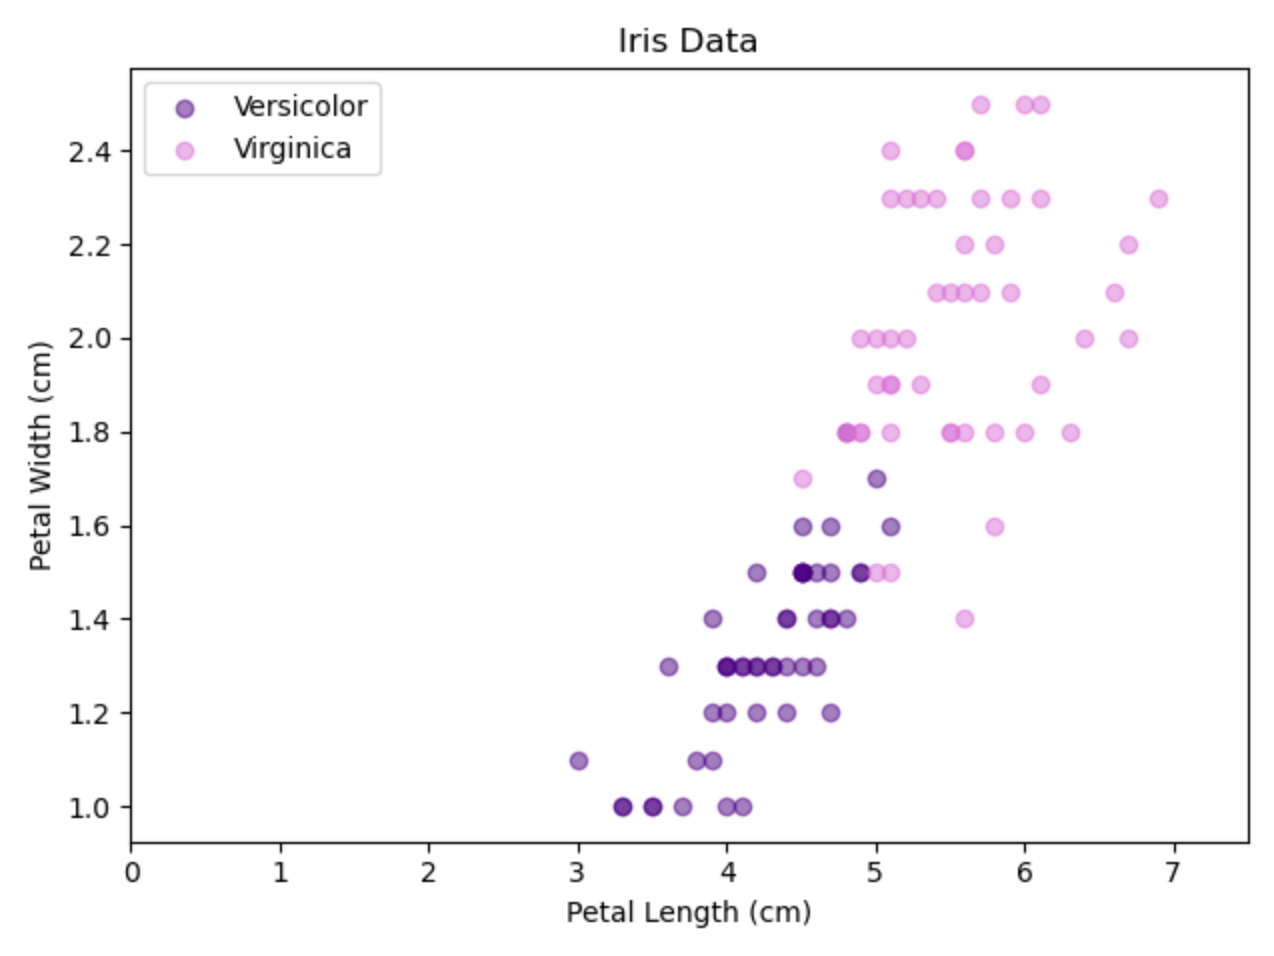
\includegraphics[scale=0.40]{1a_plot.png}
\end{center}
\subsection*{b)}
We write our function abstractly as two parts:
\begin{equation*}
    \sigma(y)=\frac{1}{1+e^{-y}}\text{, where }y=\mathbf{m}^{T}\mathbf{x}+b =m_{1}x_{1} + m_{2}x_{x} + b
\end{equation*}
where $\mathbf{x}$ is the data vector $=\begin{Bmatrix}x_{1}=\text{petal length}\\x_{2}=\text{petal width}\end{Bmatrix}$ and $y$ is the output value.\\
\subsection*{c)}
For the parameters, I chose $\mathbf{m}=\begin{bmatrix}0.6\\1.8\end{bmatrix}$ and $b=-5.73$
\begin{center}
    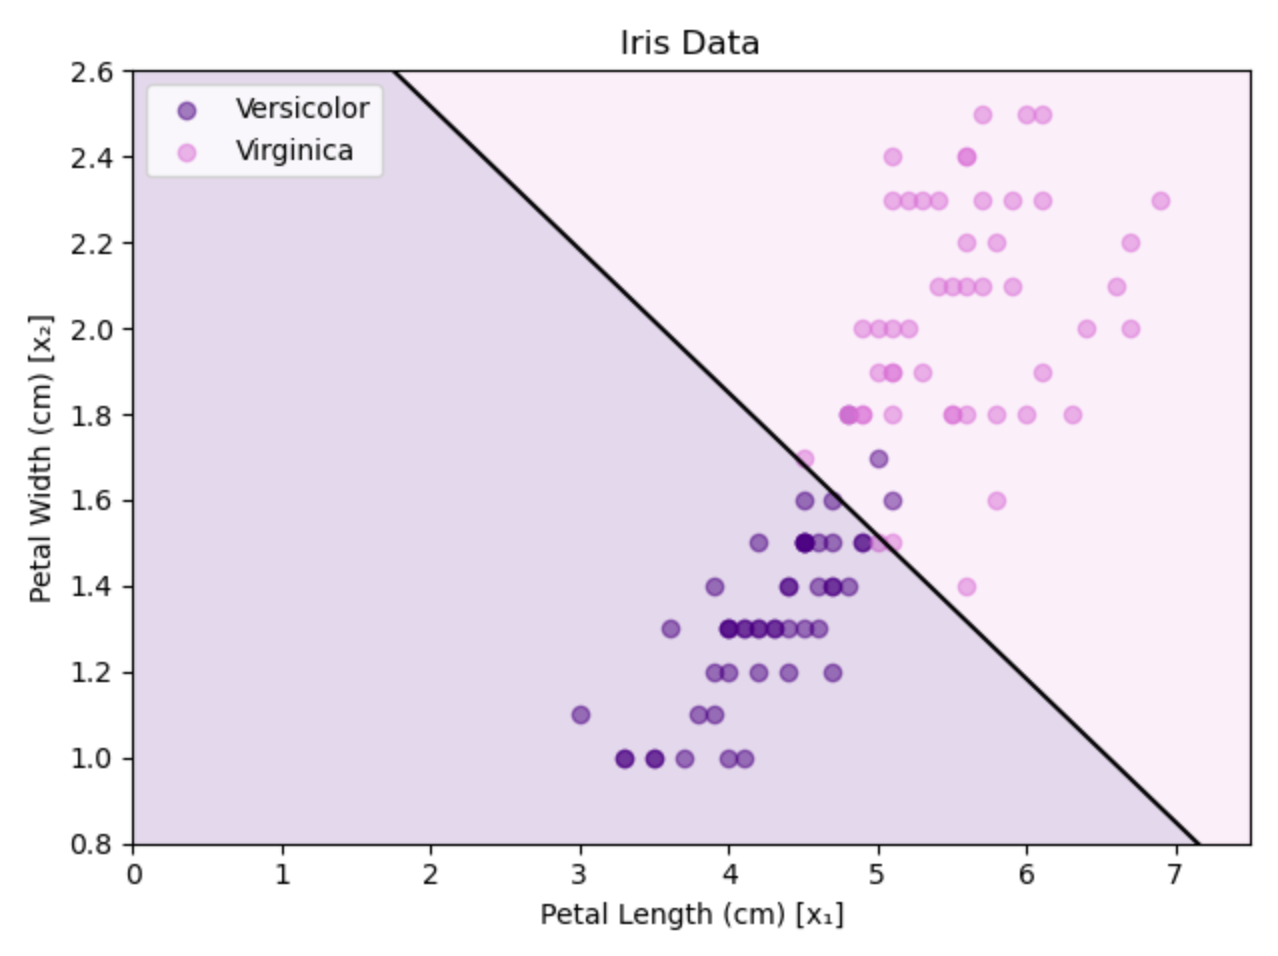
\includegraphics[scale=0.40]{1c_plot_colored.png}
\end{center}
\subsubsection*{Code:}
In \texttt{johnmays\us P2/exercise\us one.py}, refer to \texttt{plot\char`_iris\char`_data\char`_with\char`_decision\char`_boundary($\hdots$)}, a function incredibly close to \texttt{plot\char`_iris\char`_data($\hdots$)}, which I used for part \textbf{1a}.  (This creates the plot above)\\
Additionally, refer to \texttt{simple\char`_classifier(x\char`_one, x\char`_two)}, which is the function that actually returns a sigmoid value given input data $\mathbf{x}$.
\subsection*{d)}
\begin{center}
    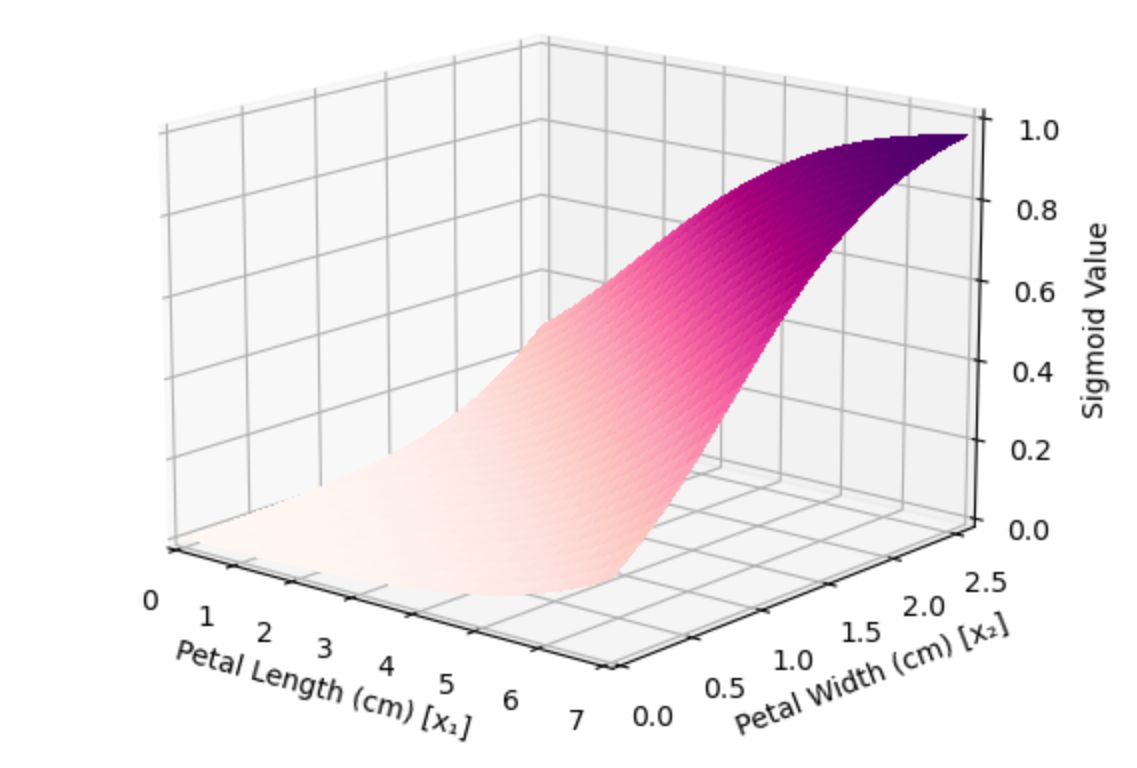
\includegraphics[scale=0.5]{1d_plot.png}
\end{center}
\subsubsection*{Code:}
Refer to \texttt{johnmays\us P2/exercise\us one.py/surface\char`_plot\char`_input\char`_space($\hdots$)}, which plots this figure.
\subsection*{e)}
For this question, I wrote a function that, for one data point, prints the petal length, petal width, true species, and simple classifier output.  The function is \texttt{test\char`_simple\char`_classifier($\hdots$)} and, given a CSV row index, calls \texttt{simple\char`_classifier(x\char`_one, x\char`_two)} on that data, and prints the required output.\\
Both functions can be found in \texttt{johnmays\us P2/exercise\us one.py}
\subsubsection*{Output and Results: }
\textbf{Unambiguously Versicolor:}\\
\texttt{Petal Length: 4.7 , Petal Width: 1.4 ,\\ True Class: \underline{versicolor} , Simple Classifier Output: 0.4037 (\underline{versicolor})\\
Petal Length: 3.5 , Petal Width: 1.0 ,\\ True Class: \underline{versicolor} , Simple Classifier Output: 0.1382 (\underline{versicolor})\\
Petal Length: 3.8 , Petal Width: 1.1 ,\\ True Class: \underline{versicolor} , Simple Classifier Output: 0.1869 (\underline{versicolor})\\
}
\textbf{Unambiguously Virginica:}\\
\texttt{Petal Length: 6.0 , Petal Width: 2.5 ,\\ True Class: \underline{virginica} , Simple Classifier Output: 0.9145 (\underline{virginica})\\
Petal Length: 5.7 , Petal Width: 2.3 ,\\ True Class: \underline{virginica} , Simple Classifier Output: 0.8618 (\underline{virginica})\\
Petal Length: 5.6 , Petal Width: 2.4 ,\\ True Class: \underline{virginica} , Simple Classifier Output: 0.8754 (\underline{virginica})\\
}
\textbf{Near the Decision Boundary:}\\
\texttt{Petal Length: 4.5 , Petal Width: 1.7 ,\\ True Class: \underline{virginica} , Simple Classifier Output: 0.5075 (\underline{virginica})\\
Petal Length: 5.0 , Petal Width: 1.5 ,\\ True Class: \underline{virginica} , Simple Classifier Output: 0.4925 (\underline{versicolor})\\
Petal Length: 5.1 , Petal Width: 1.6 ,\\ True Class: \underline{versicolor} , Simple Classifier Output: 0.5523 (\underline{virginica})
}\\
\linebreak
% \begin{center}
%     More remarks on next page $\rightarrow$
% \end{center}
% \pagebreak
\subsubsection*{Conclusion: }
The classifier returns expected outputs closer to 1 and 0 for the unambiguous data points, but for those near the decision boundary, I chose a virginica (the second one listed) and a versicolor that were both misclassified by the classifier, and another virginica (the first one listed) that was close, but successfully classified.  The actual value returned by the classifier for the ambiguous data points is much closer to $0.5$.
\subsubsection*{Data Used: }
I plotted the nine data points I used for convenience:
\begin{center}
    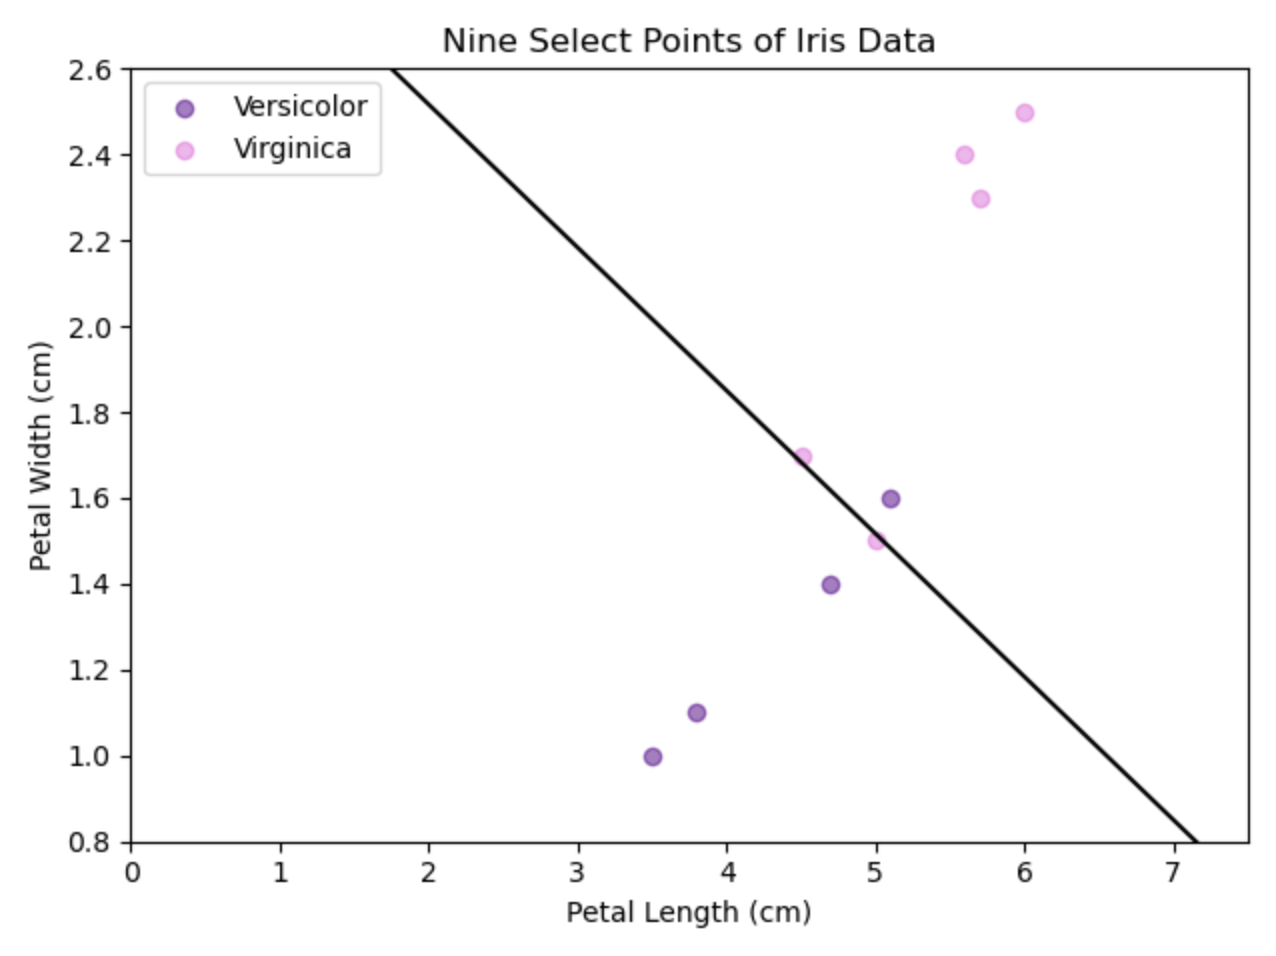
\includegraphics[scale=0.40]{1e_plot.png}
\end{center}
These data points can be found at CSV rows (beginning at $0$ with the first setosa) $50$, $60$, $80$, $100$, $120$, $140$, $106$, $119$, and $83$.
\section*{Exercise 2: Neural networks}
\subsection*{a)}
My code essentially calculates this sum:
\begin{equation*}
    \frac{1}{n}\sum_{i=1}^{n}(\text{class}(\mathbf{x_{i}})-\text{prediction}(\mathbf{x_{i}}))^{2}
\end{equation*}
My code contains a lot of extraneous information, so I will refer you to\\ \texttt{johnmays\us P2/exercise\char`_two.py/mse(X, m, b, species)}, and include my pseudocode instead:\\
\linebreak
\textsc{MSE}($\mathbf{X}$, $\mathbf{m}$, $b$, $species$)\\
\indent $sum = 0$\\
\indent \textbf{for} column vectors: $\mathbf{x}$ in $\mathbf{X}$\\
\indent \indent $sum = sum + (\text{binary value corresponding to }\mathbf{x}\text{'s }species  - \textsc{Classifier}(\mathbf{x}))^{2}$\\
\indent return $sum \div$columns in $\mathbf{X}$
\pagebreak
\subsection*{b)}
For a good choice of parameters, I chose what I used in part \textbf{1c}: $\mathbf{m}=\begin{bmatrix}0.6\\1.8\end{bmatrix}$ and $b=-5.73$\\
For a bad choice, I chose: $\mathbf{m}=\begin{bmatrix}1.0\\2.1\end{bmatrix}$ and $b=-6$.\\
\linebreak
Both decision boundaries are plotted here:
\begin{center}
    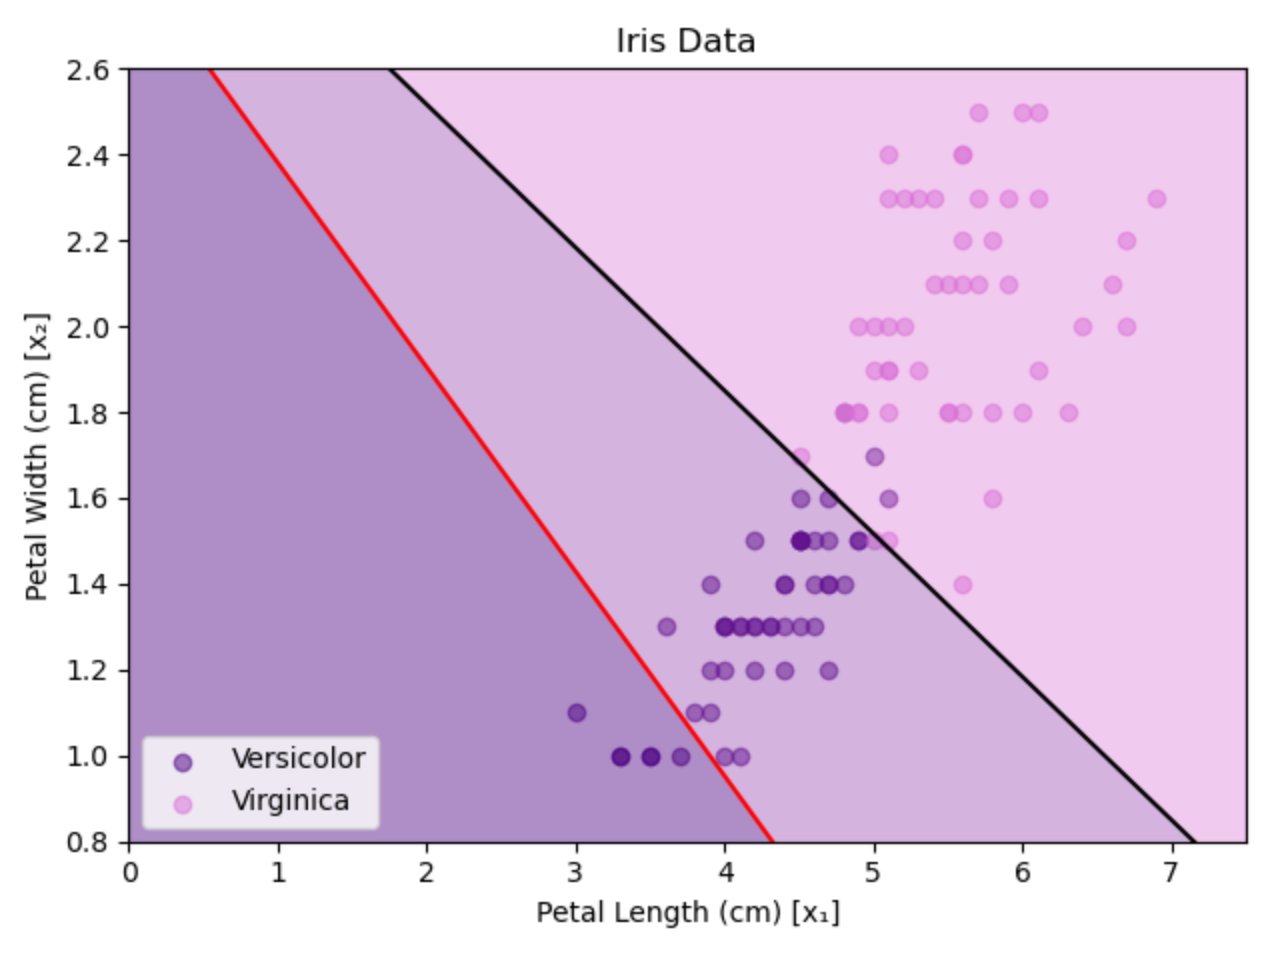
\includegraphics[scale = 0.4]{2b_plot_2.png}
\end{center}
The original one (black) does a good job splitting the data, but the bad one (\textcolor{red}{red}) accurately classifies only a little more than half of the of the data.\\
\subsubsection*{Results}
Calling my \texttt{mse($\hdots$)} function with the good parameters returned a mean squared error of $0.0969$.\\
Calling it with the bad parameters returned a mean squared error of $0.2688$.  Looking at the bad decision boundary, this makes sense, as around half of the data points (mostly virginica and a few versicolor) will be mostly well-classified; however, a large chunk of versicolors are close to the decision boundary, but are misclassified.
\subsubsection*{Code:}
In \texttt{johnmays\us P2/main.py}, there is a function called \texttt{output\us 2b()} that, when itself called, will call the appropriate functions in \texttt{johnmays\us P2/exercise\us two.py} to plot the decision boundaries and print the mean-squared-error values.  Those functions are \texttt{mse($\hdots$)} and \texttt{plot\us iris\us data\us with\us two\us decision\us boundaries($\hdots$)
}
\pagebreak
\subsection*{c)}
\subsubsection*{Setting up the Problem:}
With respect to one input data vector $\mathbf{x}=\begin{bmatrix}1\\x_{1}\\x_{2}\end{bmatrix}$, the \underline{objective function}, which we want to decrease is the mean squared error:
\begin{equation*}
    \textsc{MSE}(\mathbf{x}) = (\text{class}(\mathbf{x})-\text{prediction}(\mathbf{x}))^{2} 
\end{equation*}
\linebreak
To put it in a mathematical form, we will say we have the variables:\\
\linebreak
$y(\mathbf{x})=$ the true class, $\boldsymbol{\omega}=\begin{bmatrix}\omega_{0}\\\omega_{1}\\\omega_{2}\end{bmatrix}=$ the weights, $\mathbf{x}=\begin{bmatrix}1\\x_{1}\\x_{2}\end{bmatrix}=$ the input data,\\
\linebreak
and the prediction function $\sigma(\boldsymbol{\omega}^{T}\mathbf{x})=\sigma(\omega_{0}+\omega_{1}x_{1}+\omega_{2}x_{2})$.\\
\linebreak
We can therefore write out the objection function in mathematical terms as:
\begin{equation*}
    (y(\mathbf{x})-\sigma(\boldsymbol{\omega}^{T}\mathbf{x}))^{2}
\end{equation*}
\subsubsection*{Taking the partial derivative of the objective function with respect to $\omega_{i}$}
\begin{flalign*}
    \frac{\partial}{\partial \omega_{i}}(y(\mathbf{x})-\sigma(\boldsymbol{\omega}^{T}\mathbf{x}))^{2} &= 2(y(\mathbf{x})-\sigma(\boldsymbol{\omega}^{T}\mathbf{x}))\frac{\partial}{\partial \omega_{i}}(y(\mathbf{x})-\sigma(\boldsymbol{\omega}^{T}\mathbf{x})) && \textit{invoking the chain rule}\\
    &= 2(y(\mathbf{x})-\sigma(\boldsymbol{\omega}^{T}\mathbf{x}))(-\sigma'(\boldsymbol{\omega}^{T}\mathbf{x}))\frac{\partial}{\partial \omega_{i}}(\boldsymbol{\omega}^{T}\mathbf{x}) && \textit{invoking the chain rule again...}\\
    &= 2(y(\mathbf{x})-\sigma(\boldsymbol{\omega}^{T}\mathbf{x}))(-\sigma'(\boldsymbol{\omega}^{T}\mathbf{x})) x_{i} && \\
    &= -2(y(\mathbf{x})-\sigma(\boldsymbol{\omega}^{T}\mathbf{x}))(\sigma(\boldsymbol{\omega}^{T}\mathbf{x})(1-\sigma(\boldsymbol{\omega}^{T}\mathbf{x})))x_{i} &&\textit{writing out $\sigma'(\mathbf{x})$}\\
    &= -2(y(\mathbf{x})-\frac{1}{1+e^{-\boldsymbol{\omega}^{T}\mathbf{x}}})(\frac{1}{1+e^{-\boldsymbol{\omega}^{T}\mathbf{x}}}(1-\frac{1}{1+e^{-\boldsymbol{\omega}^{T}\mathbf{x}}}))x_{i} &&\textit{making the $\sigma$'s explicit}\\
    &= -2(y(\mathbf{x})-\frac{1}{1+e^{-\boldsymbol{\omega}^{T}\mathbf{x}}})((\frac{1}{1+e^{-\boldsymbol{\omega}^{T}\mathbf{x}}}-\frac{1}{(1+e^{-\boldsymbol{\omega}^{T}\mathbf{x}})^2}))x_{i} &&\textit{simplifying...}\\
    &= -2(y(\mathbf{x})-\frac{1}{1+e^{-\boldsymbol{\omega}^{T}\mathbf{x}}})((\frac{1+e^{-\boldsymbol{\omega}^{T}\mathbf{x}}}{(1+e^{-\boldsymbol{\omega}^{T}\mathbf{x}})^{2}}-\frac{1}{(1+e^{-\boldsymbol{\omega}^{T}\mathbf{x}})^2}))x_{i} && \\
    &= -2(y(\mathbf{x})-\frac{1}{1+e^{-\boldsymbol{\omega}^{T}\mathbf{x}}})((\frac{e^{-\boldsymbol{\omega}^{T}\mathbf{x}}}{(1+e^{-\boldsymbol{\omega}^{T}\mathbf{x}})^2}))x_{i} && 
\end{flalign*}
Specific forms of gradient to be written out in part \textbf{2d} $\rightarrow$
% \begin{flalign*}
%     \frac{\partial \sigma(y)}{\partial \omega_{1}}
%     &= \frac{\partial \sigma(y)}{\partial y} \frac{\partial y}{\partial \omega_{1}} && \textit{invoking the chain rule}\\
%     &= \sigma(y)(1-\sigma(y)) \frac{\partial y}{\partial \omega_{1}} = \sigma(y)(1-\sigma(y)) \frac{\partial}{\partial \omega_{1}} \omega_{0}+\omega_{1}x_{1}+\omega_{2}x_{2} && \textit{writing it out...}\\
%     &=\sigma(y)(1-\sigma(y)) x_{1} && \textit{calculating the second derivative}\\
%     &= \frac{1}{1+e^{-y}}(1-\frac{1}{1+e^{-y}})x_{1} = (\frac{1}{1+e^{-y}}-\frac{1}{(1+e^{-y})^{2}})x_{1}&& \textit{cleaning up the expression...}\\
%     &= \frac{e^{-y}}{(1+e^{-y})^{2}}x_{1} && \\
%     &= \frac{x_{1}e^{-\omega_{0}-\omega_{1}x_{1}-\omega_{2}x_{2}}}{(1+e^{-\omega_{0}-\omega_{1}x_{1}-\omega_{2}x_{2}})^{2}} && \textit{writing it out explicitly}
% \end{flalign*}
\subsection*{d)}
The gradient of the objective for one weight, $\omega_{i}$ is:
\begin{align*}
    \frac{\partial}{\partial \omega_{i}}(y(\mathbf{x})-\sigma(\boldsymbol{\omega}^{T}\mathbf{x}))^{2} = -2(y(\mathbf{x})-\frac{1}{1+e^{-\boldsymbol{\omega}^{T}\mathbf{x}}})((\frac{e^{-\boldsymbol{\omega}^{T}\mathbf{x}}}{(1+e^{-\boldsymbol{\omega}^{T}\mathbf{x}})^2}))x_{i}
\end{align*}
Therefore, for the \textbf{scalar} weights, the gradient can be written as:
\begin{flalign*}
    \text{for $\omega_{0}$: }&\frac{\partial}{\partial \omega_{0}}(y(\mathbf{x})-\sigma(\boldsymbol{\omega}^{T}\mathbf{x}))^{2} = -2(y(\mathbf{x})-\frac{1}{1+e^{-\boldsymbol{\omega}^{T}\mathbf{x}}})((\frac{e^{-\boldsymbol{\omega}^{T}\mathbf{x}}}{(1+e^{-\boldsymbol{\omega}^{T}\mathbf{x}})^2}))&&\\
    \text{for $\omega_{1}$: }&\frac{\partial}{\partial \omega_{1}}(y(\mathbf{x})-\sigma(\boldsymbol{\omega}^{T}\mathbf{x}))^{2} = -2(y(\mathbf{x})-\frac{1}{1+e^{-\boldsymbol{\omega}^{T}\mathbf{x}}})((\frac{e^{-\boldsymbol{\omega}^{T}\mathbf{x}}}{(1+e^{-\boldsymbol{\omega}^{T}\mathbf{x}})^2}))x_{1}&&\\
    \text{for $\omega_{2}$: }&\frac{\partial}{\partial \omega_{2}}(y(\mathbf{x})-\sigma(\boldsymbol{\omega}^{T}\mathbf{x}))^{2} = -2(y(\mathbf{x})-\frac{1}{1+e^{-\boldsymbol{\omega}^{T}\mathbf{x}}})((\frac{e^{-\boldsymbol{\omega}^{T}\mathbf{x}}}{(1+e^{-\boldsymbol{\omega}^{T}\mathbf{x}})^2}))x_{2}&&
\end{flalign*}
And the \textbf{vector} gradient can be written as a collection of the scalar expressions:
\begin{equation*}
    \nabla (y(\mathbf{x})-\sigma(\boldsymbol{\omega}^{T}\mathbf{x}))^{2}= 
    \begin{Bmatrix}
         \frac{\partial}{\partial \omega_{0}}\\
         \frac{\partial}{\partial \omega_{1}}\\
         \frac{\partial}{\partial \omega_{2}}
    \end{Bmatrix}=
    \begin{Bmatrix}
         -2(y(\mathbf{x})-\frac{1}{1+e^{-\boldsymbol{\omega}^{T}\mathbf{x}}})((\frac{e^{-\boldsymbol{\omega}^{T}\mathbf{x}}}{(1+e^{-\boldsymbol{\omega}^{T}\mathbf{x}})^2}))\\
         -2(y(\mathbf{x})-\frac{1}{1+e^{-\boldsymbol{\omega}^{T}\mathbf{x}}})((\frac{e^{-\boldsymbol{\omega}^{T}\mathbf{x}}}{(1+e^{-\boldsymbol{\omega}^{T}\mathbf{x}})^2}))x_{1}\\
         -2(y(\mathbf{x})-\frac{1}{1+e^{-\boldsymbol{\omega}^{T}\mathbf{x}}})((\frac{e^{-\boldsymbol{\omega}^{T}\mathbf{x}}}{(1+e^{-\boldsymbol{\omega}^{T}\mathbf{x}})^2}))x_{2}
    \end{Bmatrix}
\end{equation*}
\subsection*{e)}
I began with weight vector $\boldsymbol{\omega}=\begin{bmatrix}\omega_{0}\\\omega_{1}\\\omega_{2}\end{bmatrix}=\begin{bmatrix}-4.0\\0.6\\1.8\end{bmatrix}$\\
\linebreak
Then, I ran my \texttt{gradient\us mse($\hdots$)} function and subtracted the returned gradient sum vector multiplied by a step size of $0.005$ from the original weights, to get a new weight vector: $\boldsymbol{\omega}=\begin{bmatrix}-4.0636\\0.3320\\1.7173\end{bmatrix}$\\
\linebreak
\textbf{Here are the first and second weights' decision boundaries plotted:}
\begin{center}
    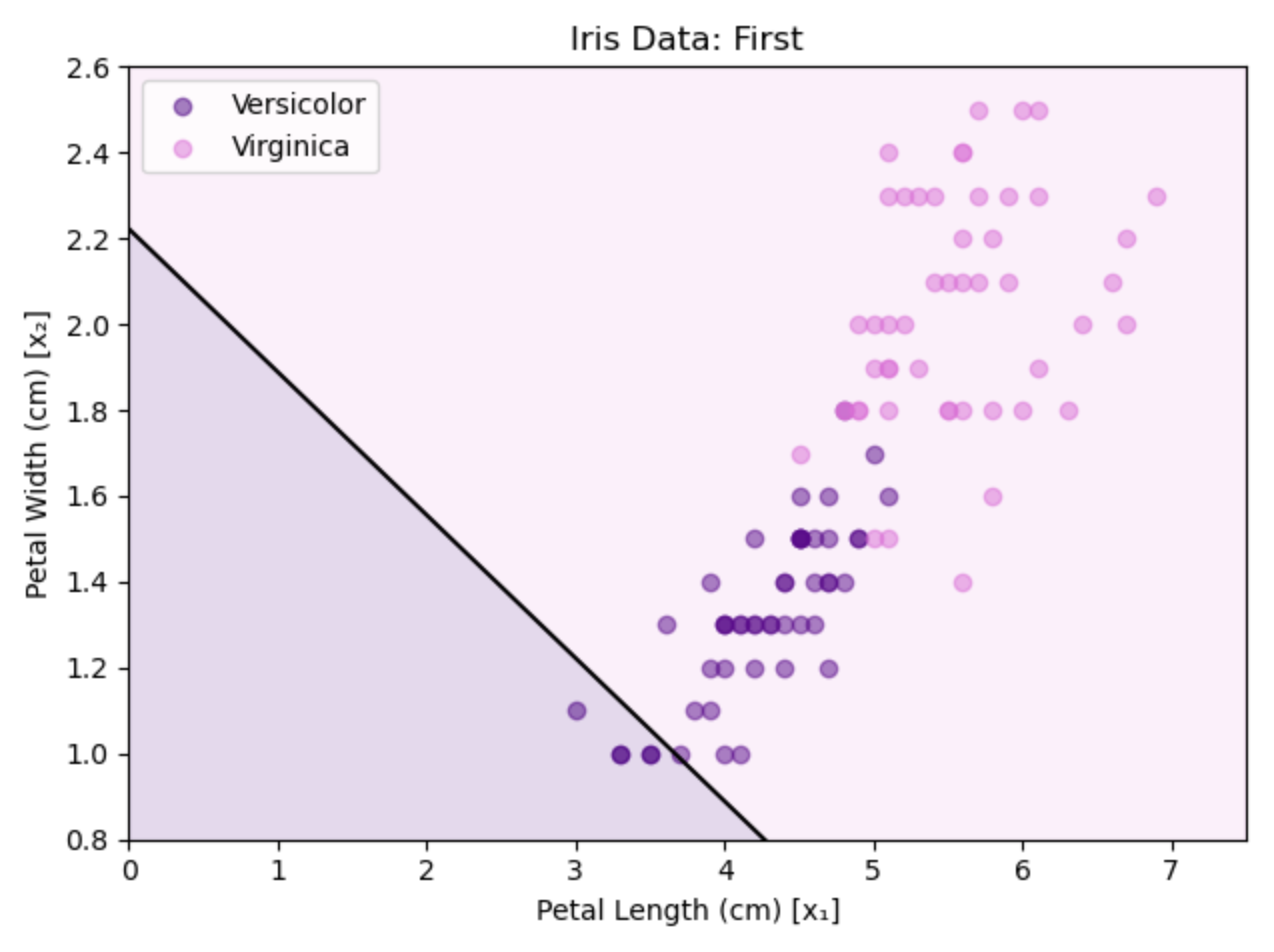
\includegraphics[scale = 0.32]{2e_plot_1.png}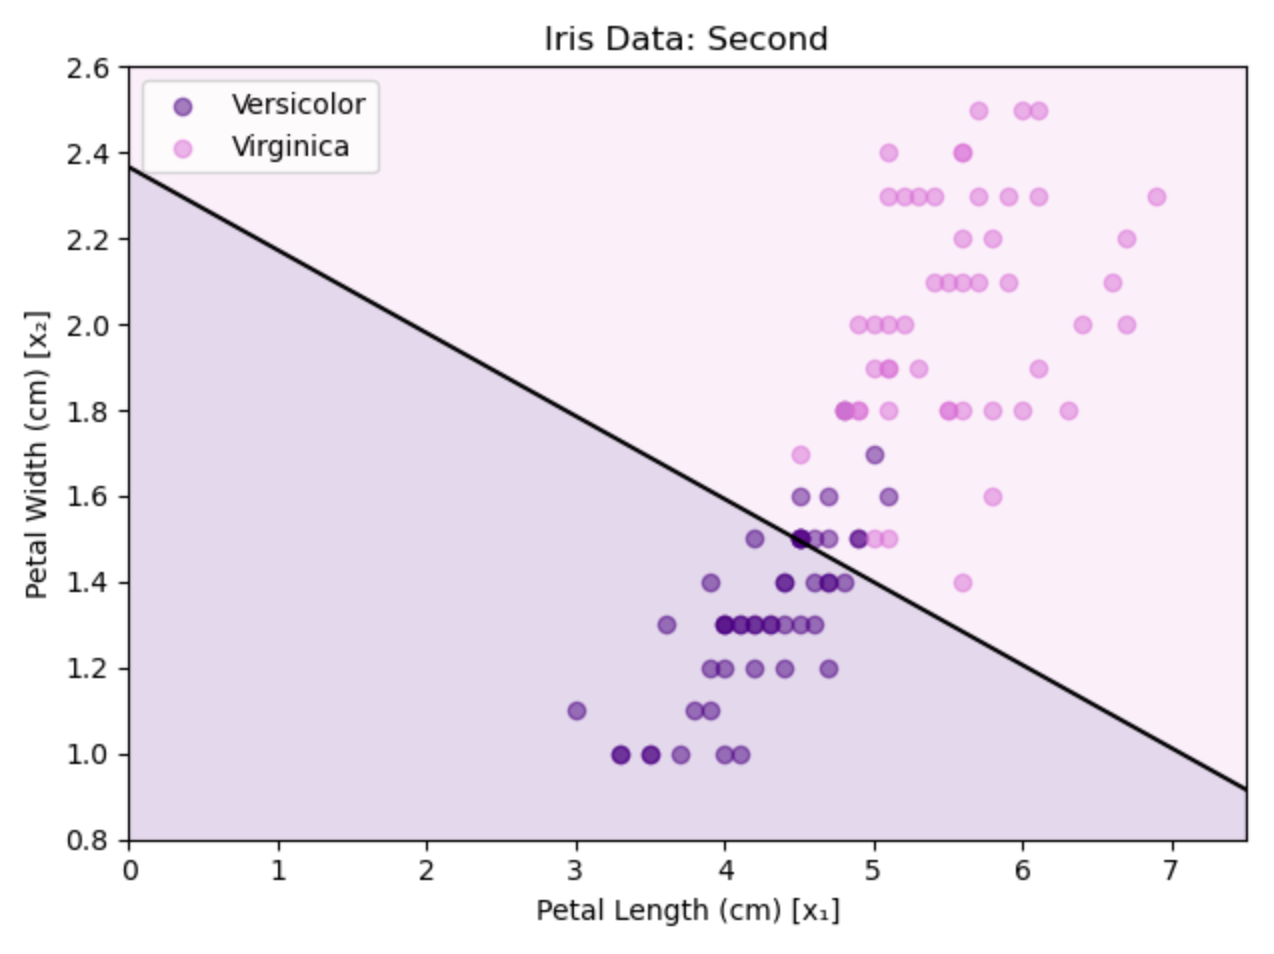
\includegraphics[scale = 0.32]{2e_plot_2.png}
\end{center}
\subsubsection*{Code:}
In \texttt{johnmays\us P2/main.py}, there is a function called \texttt{output\us 2e()} that, when itself called, will call a sequence of functions that produce the above output.\\
\linebreak
The function that actually computes the gradient for a batch of data can be found in \texttt{johnmays\us P2/exercise\us two.py} and is called \texttt{gradient\us mse($\hdots$)}.  As its input, it takes a matrix of $3\times 1$ data vectors (with the first entry always being 1), a $3\times 1$ weight vector, and the vector $species$, which contains the ground truth for all of the data points.\\
\linebreak
To make the plots, I simply call \texttt{plot\us iris\us data\us with\us decision\us boundary($\hdots$)} from part \textbf{1c}. 
\pagebreak
\section*{Exercise 3: Learning a decision boundary \\through optimization}
\subsection*{a)}
In \texttt{johnmays\us P2/exercise\us three.py}, I wrote a function called \texttt{fit($\hdots$)}, that implements gradient descent.\\
\linebreak
To \texttt{fit($\hdots$)}, I pass the $X$ matrix containing $100$ $3 \times 1$ data vectors, the step size variable, and a \texttt{simple\us classifier($\hdots$)} model object that I instantiate with the starting weights beforehand.  I also pass it the data vectors \texttt{petal\us length}, \texttt{petal\us width}, and \texttt{species} so that it can easily generate the required plots for the next section, \textbf{3b}.\\
\linebreak
In addition to producing the appropriate plots (only if you tell it to by passing the argument \texttt{progress\us output}$=$\texttt{True}), the \texttt{fit($\hdots$)} function simply returns a final weights vector.
\subsection*{b)}
When calling the \texttt{fit($\hdots$)} function mentioned in \textbf{3a}, if you pass the argument \texttt{progress\us output}$=$\texttt{True}, the function will, after learning
\begin{itemize}
    \item make three decision boundary plots for the first, middle, and last iteration, by calling the\\ \texttt{plot\us iris\us data\us with\us decision\us boundary($\hdots$)} function from \texttt{johnmays\us P2/exercise\us one.py} three times.
    \item plot the mean squared error (loss) over number of iterations by calling\\ \texttt{johnmays\us P2/exercise\us three.py/plot\us loss\us over\us iterations($\hdots$)}.
\end{itemize}
\subsection*{c)}
To begin, I call \texttt{johnmays\us P2/exercise\us three.py/random\us weights($\hdots$)} to give me a random starting vector.  It gave me $\boldsymbol{\omega}=\begin{bmatrix}-3.4153\\-0.4774\\-3.2777\end{bmatrix}$\\
I then instantiate a \texttt{simple\us classifier($\hdots$)} object with the random weights, and call \texttt{fit($\hdots$, progress\us output=True)}, which makes plots for three stages of learning.  Here is an example run based on the above random weights:
\subsubsection*{Initial: }
\begin{center}
    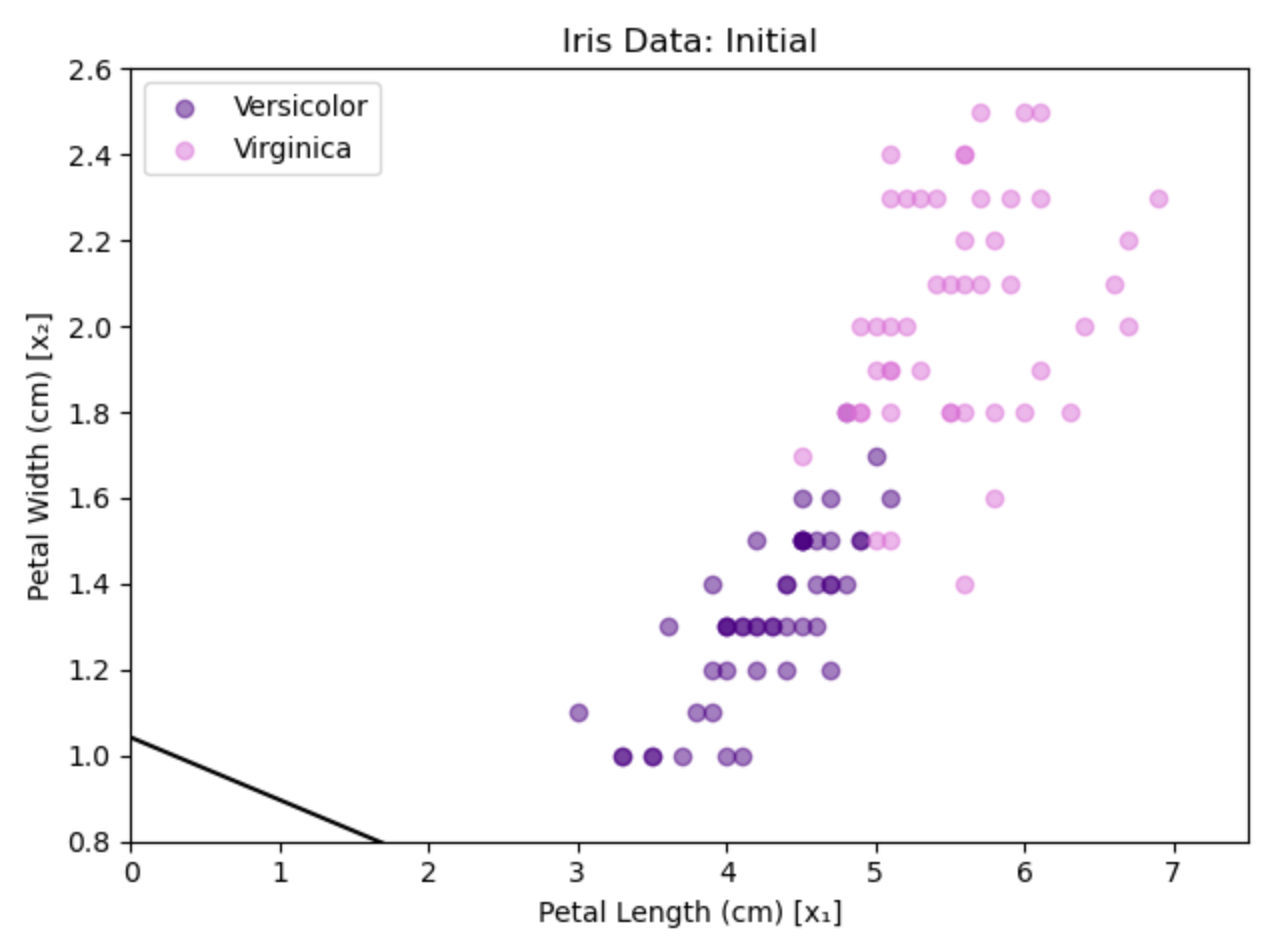
\includegraphics[scale = 0.35]{3c_plot_initial_db.png} \textit{no loss graph because it would be empty at the beginning}
\end{center}
\subsubsection*{Middle: }
\begin{center}
    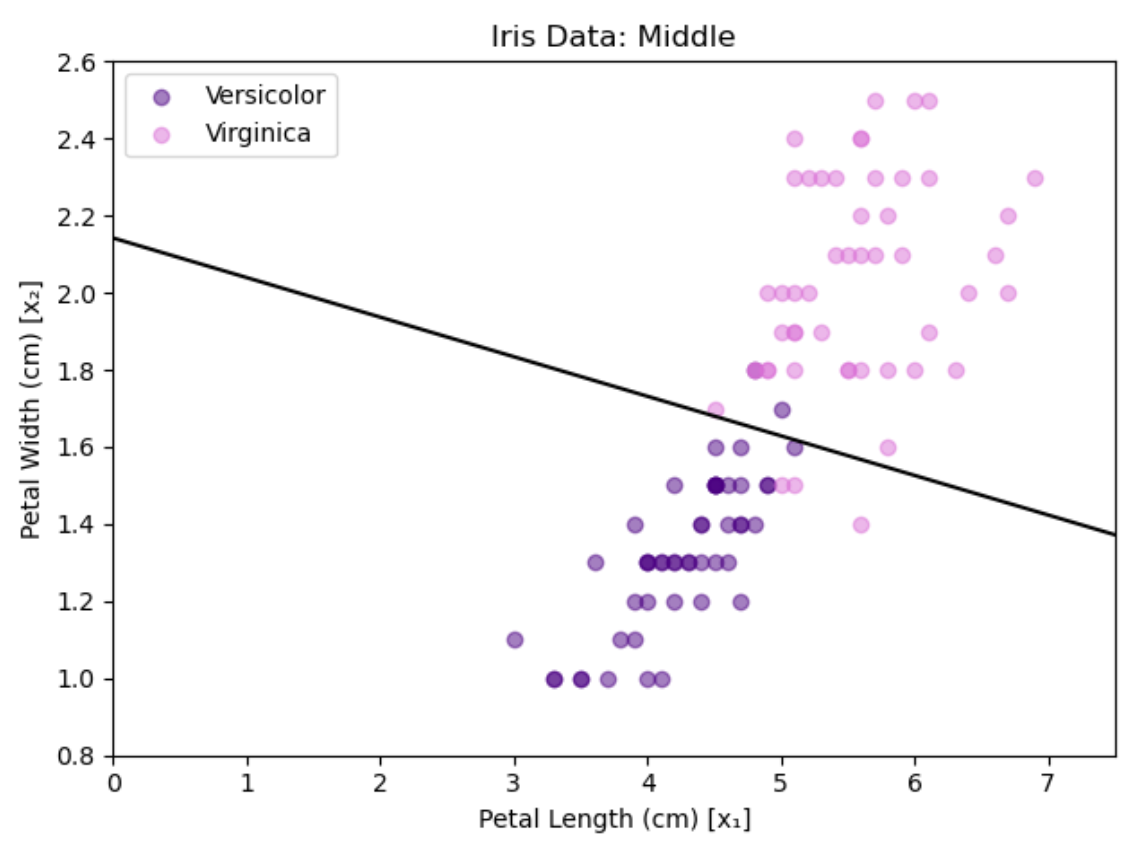
\includegraphics[scale = 0.388]{just_another_screenshot.png} 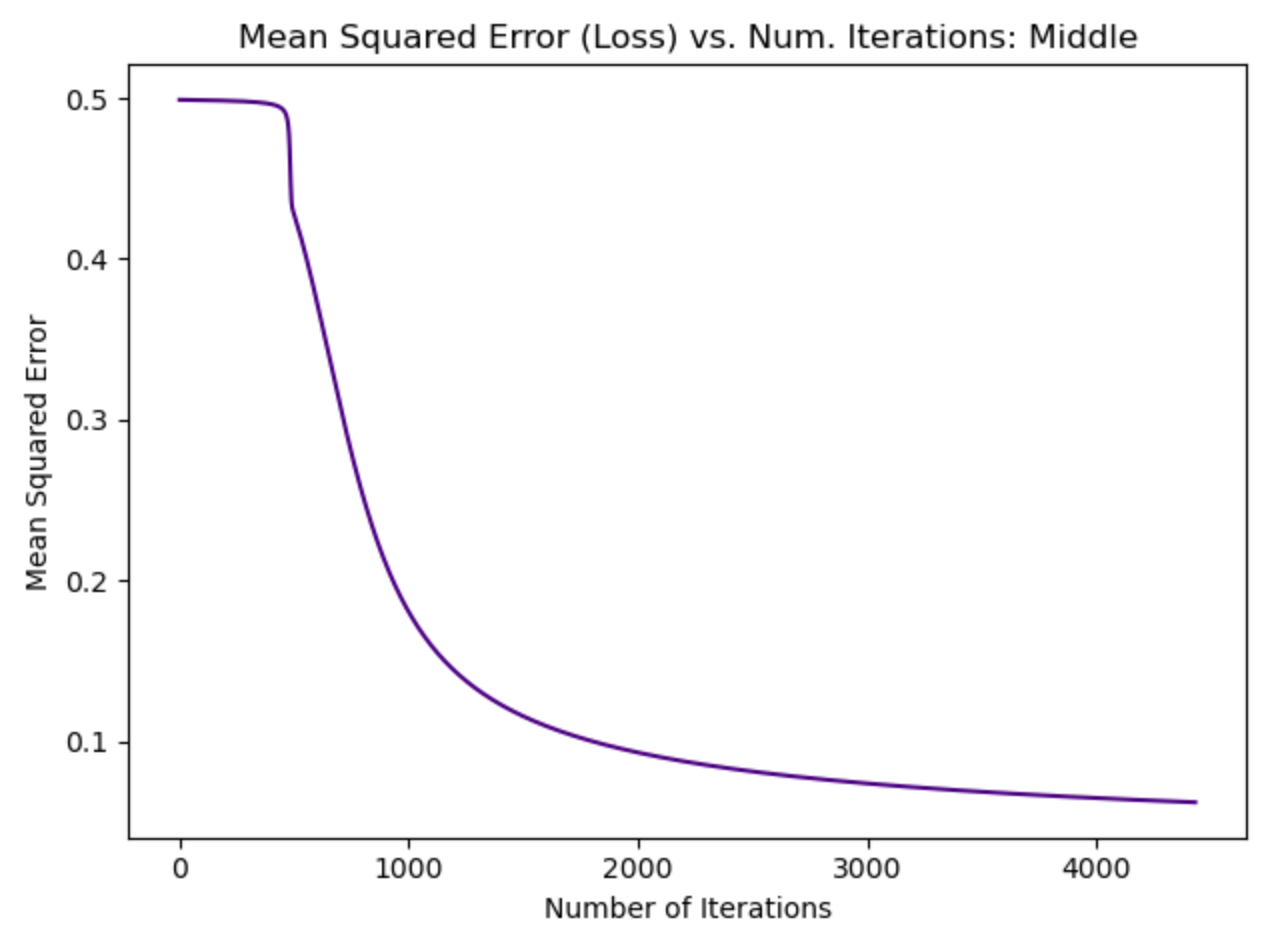
\includegraphics[scale = 0.35]{3c_plot_middle_loss.png}
\end{center}
\subsubsection*{Final: }
\begin{center}
    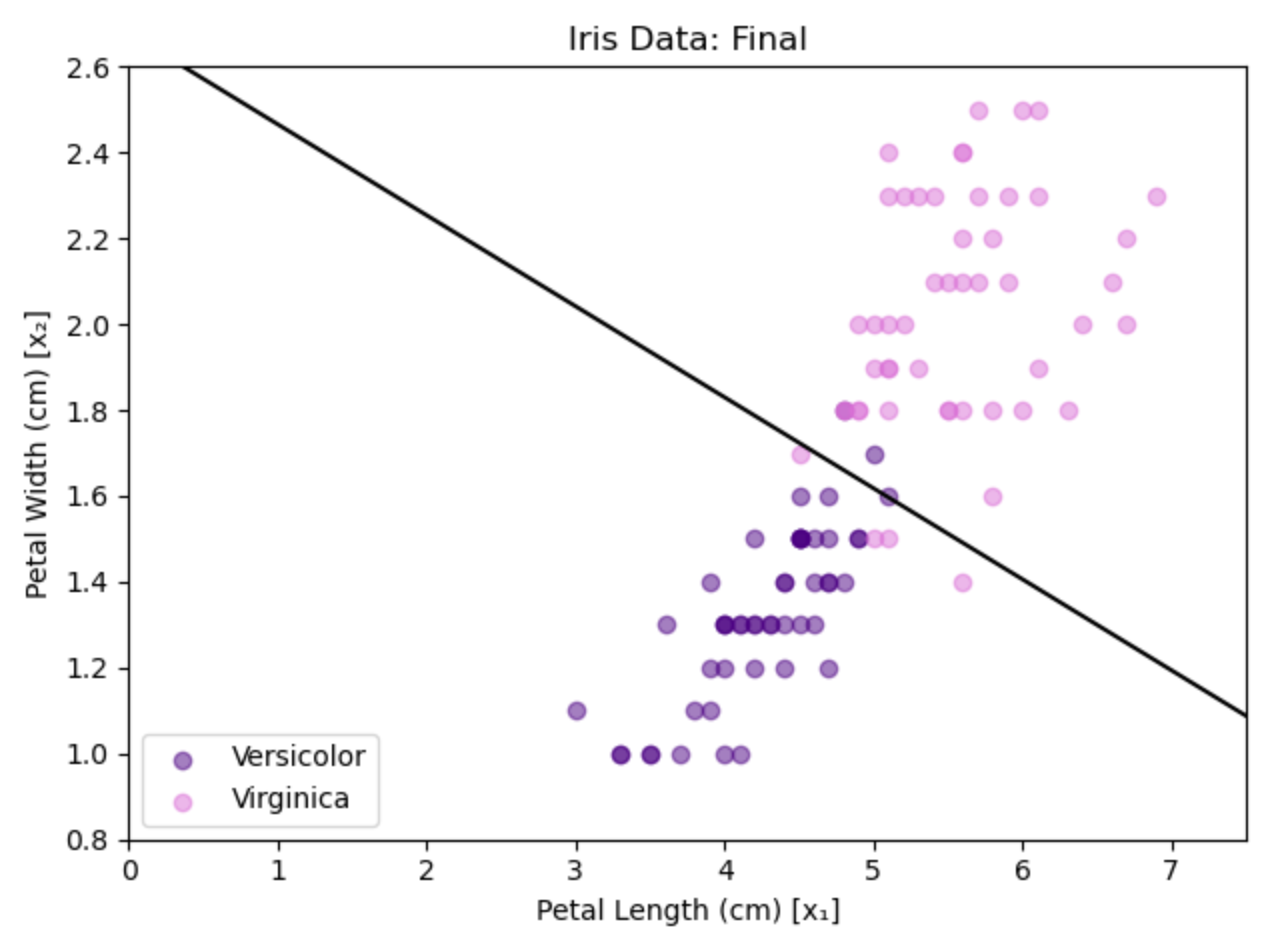
\includegraphics[scale = 0.35]{3c_plot_final_db.png} 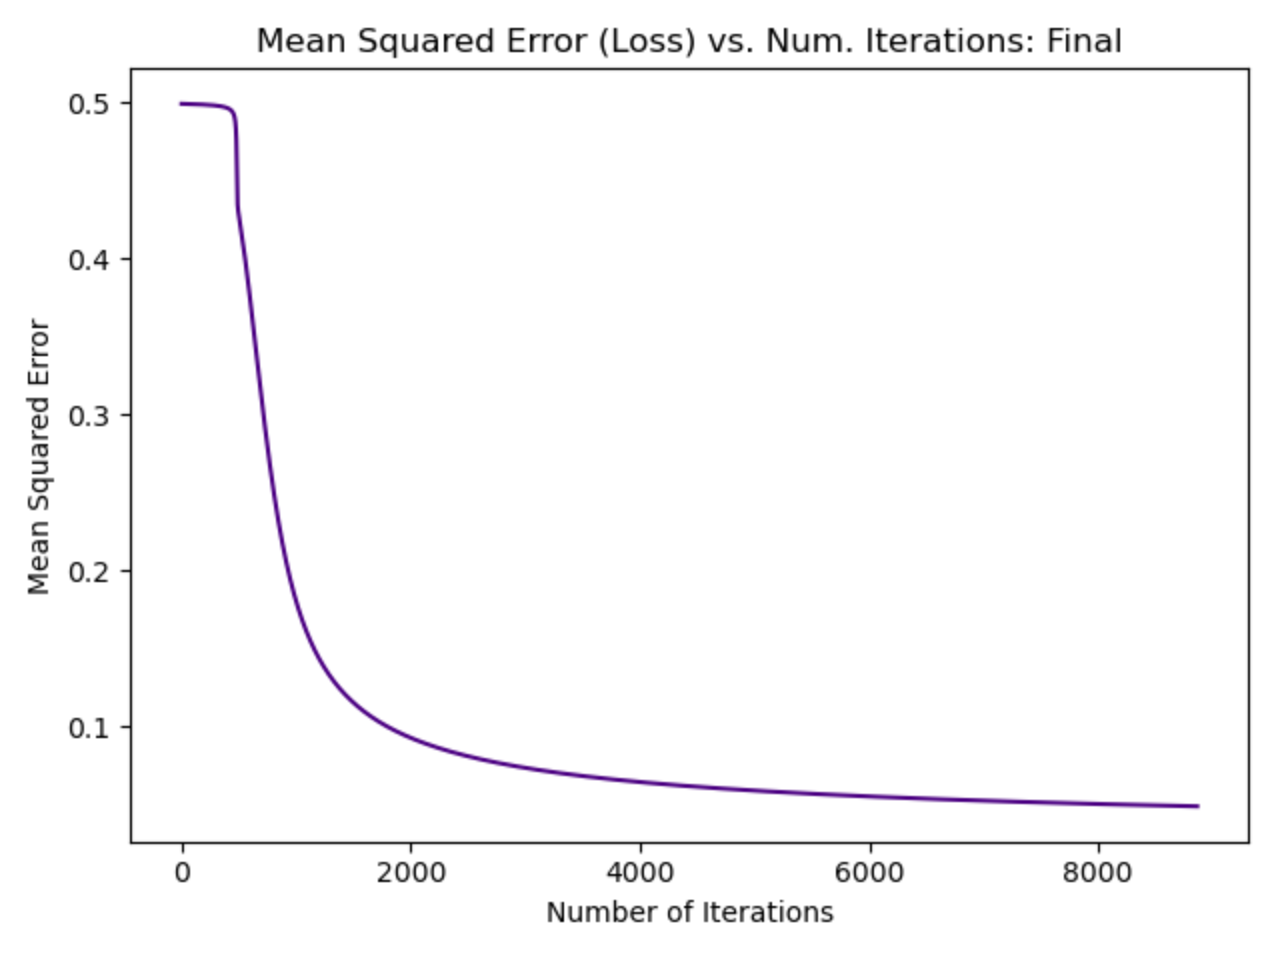
\includegraphics[scale = 0.35]{3c_plot_final_loss.png}
\end{center}
\subsubsection*{Results:}
The \texttt{fit($\hdots$)} function, once converged, returns a final weight vector of $\boldsymbol{\omega}=\begin{bmatrix}-12.8066\\1.0138\\4.7827\end{bmatrix}$
\subsubsection*{Code:}
From \texttt{johnmays\us P2/main.py}, this entire process can be run just with the command \texttt{output\us 3c()}.  This command relies on the functions described just above, which can be located in \texttt{johnmays\us P2/exercise\us three.py}.

\subsection*{d)}
I landed on \texttt{step\us size}$=\alpha=0.0025$.\\
\linebreak
The objective of setting the correct step size is, given a range of gradient values, to approach the minimum loss slowly enough that you do not overshoot.  Given this criteria, you could set it very small, but the smaller it is, the more computing resources are used.\\
Therefore I, being familiar with typical step sizes as values around $[0.01,0.0001]$. started with $0.0001$, which took longer than I was willing to wait.  Therefore I increased it to $0.01$, but that let to very wonky behavior in the loss graphs, so I settled on the order of $0.001$, and fine-tuned it until I thought the loss graphs were easy to read.
\subsection*{e)}
Theoretically speaking, the stopping criterion is when $|\nabla\textsc{MSE}|=0$.  However, I knew that was probably unrealistic considering step size is not infinitesimal, there are rounding errors, etc.  So I decided to test values for a threshold such that the fitting would stop when $|\nabla\textsc{MSE}|$ is less than the threshold.  Inspecting my loss vs. number of iterations graphs, the change in loss plateaued over time, and a threshold value of $0.25$ seemed to eliminate most of the redundant plateauing.

\end{document}